\documentclass{article}
\usepackage{amsthm}
\usepackage{amsmath}
\usepackage{tikz}
\usepackage{pgfmath}
\usetikzlibrary{positioning, arrows,automata}
\usetikzlibrary{shapes}

\begin{document}
\section {Flow Chart}
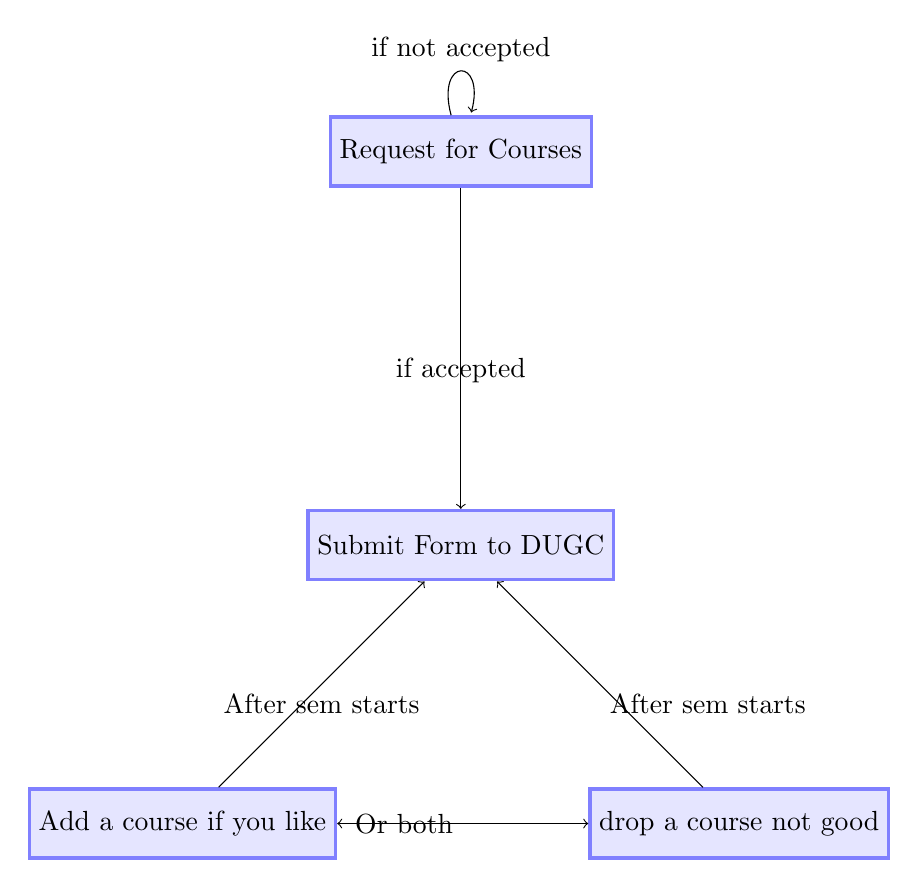
\begin{tikzpicture}[node distance=5cm, auto]
  \tikzstyle{every state}=[draw=blue!50, very thick, fill=blue!10];
  \node [state,shape=rectangle] at (0,0)             (Request)   {Request for Courses};
  \node [state,shape=rectangle, below of= Request]          (Submit)    {Submit Form to DUGC};
  \node [state,shape=rectangle, below left of= Submit]        (Add)       {Add a course if you like};
  \node [state,shape=rectangle, below right of= Submit]        (Drop)      {drop a course not good};

  \path[->] (Request) edge node[below]{if accepted} (Submit);

  \path[<-] (Submit) edge node[below]{After sem starts} (Add)
                 edge node[below right]{After sem starts} (Drop);
\path[->] (Request) edge [loop above] node {if not accepted} ();

  \path[<->] (Drop) edge node[left]{Or both} (Add);
\end{tikzpicture}
\end{document}
